Inspired by the FloPoCo~\cite{8877424} project, whose floating point (FP) arithmetic core generators we employ, our design methodology can best be described as \emph{computing just right}; 
we aim for just the right amount of compute and abstraction for the task at hand, no more, no less.
This methodology stands in contrast to the design methodologies of architecture designers for commodity hardware accelerators (such as GPUs), which must support a large set of use cases.
Accordingly, our methodology consists of five techniques distilled from such general purpose architectures and tools but specialized for our specific purposes.

\subsection{Abstract Interpretation for Efficient Transformations}\label{subsec:loop-unrolling}

It is well known that the most straightforward way to achieve lowest latency inference of a DNN is to linearize the control flow graph~\cite{osti_1574050} (i.e., remove branches) and flatten the dataflow graph as much as possible~\cite{10.1145/3295500.3356173} (i.e., execute as many operations in parallel as possible).
For intermediate level representations of a DNN, this corresponds to loop unrolling followed by fusion (alternatively known as unroll and jam~\cite{thomas1971catalogue}).
For example, consider the pair of loop nests in Listing~\ref{lst:loop_fusion}, corresponding to \texttt{Conv2d(out\_channels=64, in\_channels=1, kernel=3)}.
General purpose compilers can readily unroll each of the loop nests, but prior to fusion, due to their conservative correctness guarantees, are bound to verify that memory independence constraints are satisfied for all pairs of stores and loads in each of the loop nests.
Thus, after unrolling the inner loops of the second loop nest (on \texttt{\%i5}, \texttt{\%i6}, \texttt{\%i7}) we incur
\[
	\mathtt{\%c1} \times \mathtt{\%c3} \times \mathtt{\%c3} \times 2 \times 4
\]
memory independence checks.
Consequently, unroll and fuse optimizations take increasingly longer as one experiments with larger and larger unroll thresholds; the \emph{unroll threshold} determines which loops will be fully unrolled (all loops with trip count less than or equal to the threshold will be unrolled).
\begin{mylisting}{Loop fusion and unrolling example, for loops corresponding to \texttt{Conv2d(64, 1, 3)}, with \hl{emphasis} on loads and stores whose independence must be verified.}
	\definecolor{color02}{rgb}{0.00,0.00,0.35}
\definecolor{color05}{rgb}{0.05,0.27,0.65}
\definecolor{color06}{rgb}{0.32,0.24,0.09}
\definecolor{color07}{rgb}{0.11,0.35,0.45}
\definecolor{color08}{rgb}{0.08,0.40,0.21}
\definecolor{color09}{rgb}{0.00,0.00,1.00}
\definecolor{color10}{rgb}{0.60,1.00,0.57}


{\color{color02} \%weight} = {\color{color05} memref.get\_global} {\color{color06} @c1} 
: {\color{color07} memref}\texttt{<}{\color{color08} 64}x{\color{color08} 1}x{\color{color08} 3}x{\color{color08} 3}x{\color{color07} f32}\texttt{>}

{\color{color02} \%bias} = {\color{color05} memref.get\_global} {\color{color06} @c2} 
: {\color{color07} memref}\texttt{<}{\color{color08} 64}x{\color{color07} f32}\texttt{>}

{\color{color02} \%tmp} = {\color{color05} memref.alloca}() : {\color{color07} memref}\texttt{<}{\color{color08} 1}x{\color{color08} 64}x{\color{color08} 9}x{\color{color08} 9}x{\color{color07} f32}\texttt{>}

{\color{color05} scf.for} {\color{color02} \%i1} = {\color{color02} \%c0} {\color{color09} to} 
{\color{color02} \%c1} {\color{color09} step} {\color{color02} \%c1} :

{\color{color05} \,\,\,\,scf.for} {\color{color02} \%i2} = {\color{color02} \%c0} {\color{color09} to} 
{\color{color02} \%c64} {\color{color09} step} {\color{color02} \%c1} :

{\color{color05} \,\,\,\,\,\,\,\,scf.for} {\color{color02} \%i3} = {\color{color02} \%c0} 
{\color{color09} to} {\color{color02} \%c9} {\color{color09} step} {\color{color02} \%c1} 
:

{\color{color05} \,\,\,\,\,\,\,\,\,\,\,\,scf.for} {\color{color02} \%i4} = {\color{color02} \%c0} 
{\color{color09} to} {\color{color02} \%c9} {\color{color09} step} {\color{color02} \%c1} 
:

\,\,\,\,\,\,\,\,\,\,\,\,\,\,\,\,{\color{color02} \hlc[color10]{\%3}}\hlc[color10]{ = }{\color{color05} \hlc[color10]{memref.load}}\hlc[color10]{ 
}{\color{color02} \hlc[color10]{\%bias}}\hlc[color10]{[}{\color{color02} \hlc[color10]{\%i2}}\hlc[color10]{]}\,

{\color{color05} \,\,\,\,\,\,\,\,\,\,\,\,\,\,\,\,}{\color{color05} \hlc[color10]{memref.store}}\hlc[color10]{ 
}{\color{color02} \hlc[color10]{\%3}}\hlc[color10]{, }{\color{color02} \hlc[color10]{\%tmp}}\hlc[color10]{[}{\color{color02} \hlc[color10]{\%i1}}\hlc[color10]{, 
}{\color{color02} \hlc[color10]{\%i2}}\hlc[color10]{, }{\color{color02} \hlc[color10]{\%i3}}\hlc[color10]{, 
}{\color{color02} \hlc[color10]{\%i4}}\hlc[color10]{]}\,

\,\\
{\color{color05} scf.for} {\color{color02} \%i1} = {\color{color02} \%c0} {\color{color09} to} 
{\color{color02} \%c1} {\color{color09} step} {\color{color02} \%c1} :

{\color{color05} \,\,\,\,scf.for} {\color{color02} \%i2} = {\color{color02} \%c0} {\color{color09} to} 
{\color{color02} \%c64} {\color{color09} step} {\color{color02} \%c1} :

{\color{color05} \,\,\,\,\,\,\,\,scf.for} {\color{color02} \%i3} = {\color{color02} \%c0} 
{\color{color09} to} {\color{color02} \%c9} {\color{color09} step} {\color{color02} \%c1} 
:

{\color{color05} \,\,\,\,\,\,\,\,\,\,\,\,scf.for} {\color{color02} \%i4} = {\color{color02} \%c0} 
{\color{color09} to} {\color{color02} \%c9} {\color{color09} step} {\color{color02} \%c1} 
:

{\color{color05} \,\,\,\,\,\,\,\,\,\,\,\,\,\,\,\,scf.for} {\color{color02} \%i5} = {\color{color02} \%c0} 
{\color{color09} to} {\color{color02} \%c1} {\color{color09} step} {\color{color02} \%c1} 
:

{\color{color05} \,\,\,\,\,\,\,\,\,\,\,\,\,\,\,\,\,\,\,\,scf.for} {\color{color02} \%i6} = {\color{color02} \%c0} 
{\color{color09} to} {\color{color02} \%c3} {\color{color09} step} {\color{color02} \%c1} 
:

{\color{color05} \,\,\,\,\,\,\,\,\,\,\,\,\,\,\,\,\,\,\,\,\,\,\,\,scf.for} {\color{color02} \%i7} = {\color{color02} \%c0} 
{\color{color09} to} {\color{color02} \%c3} {\color{color09} step} {\color{color02} \%c1} 
:

\,\,\,\,\,\,\,\,\,\,\,\,\,\,\,\,\,\,\,\,\,\,\,\,\,\,\,\,{\color{color02} \%3} = {\color{color05} arith.addi} 
{\color{color02} \%i3}, {\color{color02} \%i6} : {\color{color07} i32}

\,\,\,\,\,\,\,\,\,\,\,\,\,\,\,\,\,\,\,\,\,\,\,\,\,\,\,\,{\color{color02} \%4} = {\color{color05} arith.addi} 
{\color{color02} \%i4}, {\color{color02} \%i7} : {\color{color07} i32}

\,\,\,\,\,\,\,\,\,\,\,\,\,\,\,\,\,\,\,\,\,\,\,\,\,\,\,\,{\color{color02} \hlc[color10]{\%5}}\hlc[color10]{ 
= }{\color{color05} \hlc[color10]{memref.load}}\hlc[color10]{ }{\color{color02} \hlc[color10]{\%inp}}\hlc[color10]{[}{\color{color02} \hlc[color10]{\%i1}}\hlc[color10]{, 
}{\color{color02} \hlc[color10]{\%i5}}\hlc[color10]{, \%}{\color{color08} \hlc[color10]{3}}\hlc[color10]{, 
\%}{\color{color08} \hlc[color10]{4}}\hlc[color10]{]\,}

\,\,\,\,\,\,\,\,\,\,\,\,\,\,\,\,\,\,\,\,\,\,\,\,\,\,\,\,{\color{color02} \hlc[color10]{\%6}}\hlc[color10]{ 
= }{\color{color05} \hlc[color10]{memref.load}}\hlc[color10]{ }{\color{color02} \hlc[color10]{\%weight}}\hlc[color10]{[}{\color{color02} \hlc[color10]{\%i2}}\hlc[color10]{, 
}{\color{color02} \hlc[color10]{\%i5}}\hlc[color10]{, }{\color{color02} \hlc[color10]{\%i6}}\hlc[color10]{, 
}{\color{color02} \hlc[color10]{\%i7}}\hlc[color10]{]}\,

\,\,\,\,\,\,\,\,\,\,\,\,\,\,\,\,\,\,\,\,\,\,\,\,\,\,\,\,{\color{color02} \hlc[color10]{\%7}}\hlc[color10]{ 
= }{\color{color05} \hlc[color10]{memref.load}}\hlc[color10]{ }{\color{color02} \hlc[color10]{\%tmp}}\hlc[color10]{[}{\color{color02} \hlc[color10]{\%i1}}\hlc[color10]{, 
}{\color{color02} \hlc[color10]{\%i2}}\hlc[color10]{, }{\color{color02} \hlc[color10]{\%i3}}\hlc[color10]{, 
}{\color{color02} \hlc[color10]{\%i4}}\hlc[color10]{]}\,

\,\,\,\,\,\,\,\,\,\,\,\,\,\,\,\,\,\,\,\,\,\,\,\,\,\,\,\,{\color{color02} \%8} = {\color{color05} arith.mulf} 
{\color{color02} \%5}, {\color{color02} \%6} : {\color{color07} f16}

\,\,\,\,\,\,\,\,\,\,\,\,\,\,\,\,\,\,\,\,\,\,\,\,\,\,\,\,{\color{color02} \%9} = {\color{color05} arith.addf} 
{\color{color02} \%7}, {\color{color02} \%8} : {\color{color07} f16}

{\color{color05} \,\,\,\,\,\,\,\,\,\,\,\,\,\,\,\,\,\,\,\,\,\,\,\,\,\,\,\,}{\color{color05} \hlc[color10]{memref.store}}\hlc[color10]{ 
}{\color{color02} \hlc[color10]{\%9}}\hlc[color10]{, }{\color{color02} \hlc[color10]{\%tmp}}\hlc[color10]{[}{\color{color02} \hlc[color10]{\%i1}}\hlc[color10]{, 
}{\color{color02} \hlc[color10]{\%i2}}\hlc[color10]{, }{\color{color02} \hlc[color10]{\%i3}}\hlc[color10]{, 
}{\color{color02} \hlc[color10]{\%i4}}\hlc[color10]{]}


	\label{lst:loop_fusion}
\end{mylisting}
\begin{mylisting}{Unrolled and fused loop-nest, for loops corresponding to \texttt{Conv2d(1, 64, 3)}, with \hl{emphasis} on which store-load forwards can be performed.}
	\definecolor{color02}{rgb}{0.05,0.27,0.65}
\definecolor{color05}{rgb}{0.00,0.00,0.35}
\definecolor{color06}{rgb}{0.00,0.00,1.00}
\definecolor{color07}{rgb}{0.60,1.00,0.57}
\definecolor{color08}{rgb}{0.08,0.40,0.21}


{\color{color02} scf.for} {\color{color05} \%i1} = {\color{color05} \%c0} {\color{color06} to} 
{\color{color05} \%c1} {\color{color06} step} {\color{color05} \%c1} :

{\color{color02} \,\,\,\,scf.for} {\color{color05} \%i2} = {\color{color05} \%c0} {\color{color06} to} 
{\color{color05} \%c64} {\color{color06} step} {\color{color05} \%c1} :

{\color{color02} \,\,\,\,\,\,\,\,scf.for} {\color{color05} \%i3} = {\color{color05} \%c0} 
{\color{color06} to} {\color{color05} \%c9} {\color{color06} step} {\color{color05} \%c1} 
:

{\color{color02} \,\,\,\,\,\,\,\,\,\,\,\,scf.for} {\color{color05} \%i4} = {\color{color05} \%c0} 
{\color{color06} to} {\color{color05} \%c9} {\color{color06} step} {\color{color05} \%c1} 
:

\,\,\,\,\,\,\,\,\,\,\,\,\,\,\,\,{\color{color05} \hlc[color07]{\%3}}\hlc[color07]{ = }{\color{color02} \hlc[color07]{memref.load}}\hlc[color07]{ 
}{\color{color05} \hlc[color07]{\%bias}}\hlc[color07]{[}{\color{color05} \hlc[color07]{\%i2}}\hlc[color07]{]}

{\color{color02} \,\,\,\,\,\,\,\,\,\,\,\,\,\,\,\,}{\color{color02} \hlc[color07]{memref.store}}\hlc[color07]{ 
}{\color{color05} \hlc[color07]{\%3}}\hlc[color07]{, }{\color{color05} \hlc[color07]{\%tmp}}\hlc[color07]{[}{\color{color05} \hlc[color07]{\%i1}}\hlc[color07]{, 
}{\color{color05} \hlc[color07]{\%i2}}\hlc[color07]{, }{\color{color05} \hlc[color07]{\%i3}}\hlc[color07]{, 
}{\color{color05} \hlc[color07]{\%i4}}\hlc[color07]{]}

\,\,\,\,\,\,\,\,\,\,\,\,\,\,\,\,...

\,\,\,\,\,\,\,\,\,\,\,\,\,\,\,\,{\color{color05} \%c2} = {\color{color02} arith.constant} {\color{color08} 2}

\,\,\,\,\,\,\,\,\,\,\,\,\,\,\,\,{\color{color05} \%38} = {\color{color02} arith.addi} {\color{color05} \%i3}, 
{\color{color05} \%c1}

\,\,\,\,\,\,\,\,\,\,\,\,\,\,\,\,{\color{color05} \%39} = {\color{color02} arith.addi} {\color{color05} \%i4}, 
{\color{color05} \%c2}

\,\,\,\,\,\,\,\,\,\,\,\,\,\,\,\,{\color{color05} \hlc[color07]{\%40}}\hlc[color07]{ = }{\color{color02} \hlc[color07]{memref.load}}\hlc[color07]{ 
}{\color{color05} \hlc[color07]{\%inp}}\hlc[color07]{[}{\color{color05} \hlc[color07]{\%i1}}\hlc[color07]{, 
}{\color{color05} \hlc[color07]{\%c0}}\hlc[color07]{, \%}{\color{color08} \hlc[color07]{38}}\hlc[color07]{, 
\%}{\color{color08} \hlc[color07]{39}}\hlc[color07]{]}

\,\,\,\,\,\,\,\,\,\,\,\,\,\,\,\,{\color{color05} \hlc[color07]{\%41}}\hlc[color07]{ = }{\color{color02} \hlc[color07]{memref.load}}\hlc[color07]{ 
}{\color{color05} \hlc[color07]{\%weight}}\hlc[color07]{[}{\color{color05} \hlc[color07]{\%i2}}\hlc[color07]{, 
}{\color{color05} \hlc[color07]{\%c0}}\hlc[color07]{, }{\color{color05} \hlc[color07]{\%c1}}\hlc[color07]{, 
}{\color{color05} \hlc[color07]{\%c2}}\hlc[color07]{]}

\,\,\,\,\,\,\,\,\,\,\,\,\,\,\,\,{\color{color05} \hlc[color07]{\%42}}\hlc[color07]{ = }{\color{color02} \hlc[color07]{memref.load}}\hlc[color07]{ 
}{\color{color05} \hlc[color07]{\%tmp}}\hlc[color07]{[}{\color{color05} \hlc[color07]{\%i1}}\hlc[color07]{, 
}{\color{color05} \hlc[color07]{\%i2}}\hlc[color07]{, }{\color{color05} \hlc[color07]{\%i3}}\hlc[color07]{, 
}{\color{color05} \hlc[color07]{\%i4}}\hlc[color07]{]}

\,\,\,\,\,\,\,\,\,\,\,\,\,\,\,\,{\color{color05} \%43} = {\color{color02} arith.mulf} {\color{color05} \%40}, 
{\color{color05} \%41}

\,\,\,\,\,\,\,\,\,\,\,\,\,\,\,\,{\color{color05} \%44} = {\color{color02} arith.addf} {\color{color05} \%42}, 
{\color{color05} \%43}

{\color{color02} \,\,\,\,\,\,\,\,\,\,\,\,\,\,\,\,}{\color{color02} \hlc[color07]{memref.store}}\hlc[color07]{ 
}{\color{color05} \hlc[color07]{\%44}}\hlc[color07]{, }{\color{color05} \hlc[color07]{\%tmp}}\hlc[color07]{[}{\color{color05} \hlc[color07]{\%i1}}\hlc[color07]{, 
}{\color{color05} \hlc[color07]{\%i2}}\hlc[color07]{, }{\color{color05} \hlc[color07]{\%i3}}\hlc[color07]{, 
}{\color{color05} \hlc[color07]{\%i4}}\hlc[color07]{]}

\,\,\,\,\,\,\,\,\,\,\,\,\,\,\,\,...


	\label{lst:storeloadforwarding}
\end{mylisting}

Following unroll and jam, we are able to perform \emph{store-load forwarding}, i.e., we are able to promote those store operations which are subsequently loaded from (with no intervening stores) to registers.
For example, consider the above fused loop nests, with the second loop nest having the inner three loops fully unrolled (see Listing~\ref{lst:storeloadforwarding}); the store operations on lines 6 and 13 can be entirely eliminated and the load operation on line 5 can be forwarded to the \texttt{arith.addf} on line 15.
Note, for each load operation that follows a store operation, a compiler must check whether the store and the load access the same location in memory, and further verify that there are no intervening store operations to the same memory address.
In general, this requires solving a system of constraints~\cite{10.2307/2322281}.
We observe that as loops are further and further unrolled, the cost of this particular optimization grows polynomially; consider a fully unrolled loop nest, with many parallel dataflows, for which a store operation in one dataflow might be forwarded across a parallel dataflow (and thus incur checks against all stores and loads in that parallel dataflow).

In principle, we might rely on MLIR or LLVM to perform each of these optimization passes.
The chief impediment to relying on these general purpose compilers for our needs is the runtime complexity of the their implementations.
For arbitrary programs this development time cost moderate, especially given that most development is done without these optimization (leaving the aggressive optimizations for release builds).
For us, given that the logic and dataflow of BraggNN is fixed (having already been iterated on), and given that we are in fact searching the design space for optimal low-level representations of the DNN, the runtimes of these optimization passes are prohibitive (taking on the order of hours and sometimes even days to complete).
Moreover, often their rigor and conservatism are unnecessary given a high-level understanding of the structure of BraggNN; for example, in the case of fully unrolling the above loop nests and forwarding from the stores during initialization to the loads during accumulation, the region within which the forward is safe is clear from the semantics of convolutions.
The loop indices and corresponding memory addresses for these safe store-load forwards are simple to compute analytically and ahead of time (even in the presence of complications such as strided tensors).

In order to avoid the runtime costs associated with these conservative optimization passes, we implement an abstract interpreter for sufficiently lowered DNNs.
Concretely, we lower BraggNN to the structured control flow (\texttt{scf}) dialect and then interpret this representation of BraggNN with alternative semantics.
Firstly, our interpreter evaluates functions of loop indices, such as 
\begin{mylistingnocap}
	\definecolor{color02}{rgb}{0.00,0.00,1.00}
\definecolor{color05}{rgb}{0.00,0.00,0.35}
\definecolor{color06}{rgb}{0.05,0.27,0.65}


{\color{color02} \#map} = {\color{color02} affine\_map}\texttt{<}({\color{color05} d0}, 
{\color{color05} d1}) -\texttt{>} ({\color{color05} d0} + {\color{color05} d1})\texttt{>}

{\color{color05} \%3} = {\color{color06} affine.apply} {\color{color02} \#map}({\color{color05} \%i3}, 
{\color{color05} \%i6})


\end{mylistingnocap}
or {\definecolor{color02}{rgb}{0.00,0.00,0.35}
\definecolor{color05}{rgb}{0.05,0.27,0.65}
\small\bf\fontfamily{qcr}\selectfont
{\color{color02} \%3} = {\color{color05} arith.addi} {\color{color02} \%i3}, {\color{color02} \%i6}}, where \texttt{\%i3}, \texttt{\%i6} are loop indices.
This enables us to determine array indices of stores and loads, such as 
\begin{mylistingnocap}
	\definecolor{color02}{rgb}{0.00,0.00,0.35}
\definecolor{color05}{rgb}{0.05,0.27,0.65}
\definecolor{color06}{rgb}{0.08,0.40,0.21}
\definecolor{color07}{rgb}{0.00,0.00,1.00}
\definecolor{color08}{rgb}{0.07,0.38,0.01}


{\color{color02} \%c0} = {\color{color05} arith.constant} {\color{color06} 0}

{\color{color02} \%c1} = {\color{color05} arith.constant} {\color{color06} 1}

{\color{color02} \%c3} = {\color{color05} arith.constant} {\color{color06} 3}

{\color{color02} \%c5} = {\color{color05} arith.constant}{\color{color06}  1.35}

{\color{color05} scf.for} {\color{color02} \%i1} = {\color{color02} \%c0} {\color{color07} to} 
{\color{color02} \%c3} {\color{color07} step} {\color{color02} \%c1} :

\,\,\,\,{\color{color08} // cast int to fp}

\,\,\,\,{\color{color02} \%2} = {\color{color05} arith.sitofp} {\color{color02} \%i1}

\,\,\,\,{\color{color02} \%3} = {\color{color05} arith.addf} {\color{color02} \%i1}, 
{\color{color02} \%c5}


\end{mylistingnocap}
Note that evaluation of such memory index arithmetic is typically deferred to runtime in conventional accelerators because of either the control flow inherent in a DNN, or simply a lack of available registers (to store the results).
Thus, we are able to precompute these indices, saving cycles, because BraggNN lacks control flow and FPGAs are abundant in registers.
Note also that we do not evaluate values corresponding to \texttt{memref.load}s, as they represent BraggNN weights or activations; our interpreter implements such values as proxy objects and merely records the arithmetic operations performed on them.

Secondly, our interpreter unrolls loops by executing them while enforcing SSA.
That is to say, for a loop whose body has repeated assignments to the same value (ostensibly violating SSA), such as 
\begin{mylistingnocap}
	\definecolor{color02}{rgb}{0.00,0.00,0.35}
\definecolor{color05}{rgb}{0.05,0.27,0.65}
\definecolor{color06}{rgb}{0.08,0.40,0.21}
\definecolor{color07}{rgb}{0.00,0.00,1.00}
\definecolor{color08}{rgb}{0.07,0.38,0.01}


{\color{color02} \%c0} = {\color{color05} arith.constant} {\color{color06} 0}

{\color{color02} \%c1} = {\color{color05} arith.constant} {\color{color06} 1}

{\color{color02} \%c3} = {\color{color05} arith.constant} {\color{color06} 3}

{\color{color02} \%c5} = {\color{color05} arith.constant}{\color{color06}  1.35}

{\color{color05} scf.for} {\color{color02} \%i1} = {\color{color02} \%c0} {\color{color07} to} 
{\color{color02} \%c3} {\color{color07} step} {\color{color02} \%c1} :

\,\,\,\,{\color{color08} // cast int to fp}

\,\,\,\,{\color{color02} \%2} = {\color{color05} arith.sitofp} {\color{color02} \%i1}

\,\,\,\,{\color{color02} \%3} = {\color{color05} arith.addf} {\color{color02} \%i1}, 
{\color{color02} \%c5}


\end{mylistingnocap}
we execute the loop and instantiate unique identifiers for the result of each operation:
\begin{mylistingnocap}
	\definecolor{color02}{rgb}{0.00,0.00,0.35}
\definecolor{color05}{rgb}{0.05,0.27,0.65}
\definecolor{color06}{rgb}{0.08,0.40,0.21}


{\color{color02} \%c0} = {\color{color05} arith.constant} {\color{color06} 0}\,

{\color{color02} \%c1} = {\color{color05} arith.constant} {\color{color06} 1}\,

{\color{color02} \%c2} = {\color{color05} arith.constant} {\color{color06} 2}\,

{\color{color02} \%c3} = {\color{color05} arith.constant} {\color{color06} 3}\,

{\color{color02} \%c5} = {\color{color05} arith.constant}{\color{color06}  1.35}

{\color{color02} \%2\_0} = {\color{color05} arith.sitofp} {\color{color02} \%c0}

{\color{color02} \%3\_0} = {\color{color05} arith.addf} {\color{color02} \%2\_0}, 
{\color{color02} \%c5}

{\color{color02} \%2\_1} = {\color{color05} arith.sitofp} {\color{color02} \%c1}

{\color{color02} \%3\_1} = {\color{color05} arith.addf} {\color{color02} \%2\_1}, 
{\color{color02} \%c5}

{\color{color02} \%2\_2} = {\color{color05} arith.sitofp} {\color{color02} \%c2}

{\color{color02} \%3\_2} = {\color{color05} arith.addf} {\color{color02} \%2\_2}, 
{\color{color02} \%c5}

{\color{color02} \%2\_3} = {\color{color05} arith.sitofp} {\color{color02} \%c3}

{\color{color02} \%3\_3} = {\color{color05} arith.addf} {\color{color02} \%2\_3}, 
{\color{color02} \%c5}


\end{mylistingnocap}
This enables us to both unroll the loop and track dataflow through arithmetic operations (see Section~\ref{subsec:parallel-toposort-scheduling}).
Finally, our interpreter reinterprets \texttt{memref}s as \emph{geometric symbol tables} (i.e., symbol tables indexed by array indices rather than identifiers/names) and stores/loads as assignments/reads to/from those symbol tables.
Such semantics, in combination with fully evaluated array indices, enable us to simultaneously track dataflow through activation buffers (which appear as \texttt{memref}s) and perform store/load forwarding.

The dataflow analysis carried out by our interpreter enables us to easily infer the flow of weights through the DNN and thus enables us to experiment with two weight storage strategies; namely we can either store weights as BRAMs, uniquely associated with a set of DSP blocks, or as a collection of free registers. 
The dataflow analysis also enables us to identify sequences of multiplications and additions and group them together such that they can be scheduled to reuse accumulator registers associated with floating point block instantiations (effectively forming a multiply-accumulator); 
indeed, this grouping is the chief optimization that enables us to efficiently map BraggNN to FPGA.
See Section~\ref{subsec:parallel-toposort-scheduling} for a discussion on the advantages of both of these.


% We also reinterpret remaining stores and loads to memory as reads and writes to registers, thus simplifying our design; such stores and loads would otherwise translate to stores and loads from Block RAM (BRAM).
% Furthermore, since BraggNN is a relatively small DNN, we inline absolutely all of the weight tensors as constants and perform \emph{constant propagation}.
% In summary our abstract interpreter performs the following transformations on the \texttt{scf} representation of BraggNN:
% \begin{enumerate}
% 	\item We completely eliminate any latency due to loading from or storing to BRAM for intermediate activations;
% 	\item We completely eliminate all logic (i.e., integer arithmetic) related to calculating memory offsets, a non-trivial reduction in instruction count and design complexity (see figure <figure> for reduction in instruction count);
% 	\item We instantiate a reduced set of floating point operation cores, and thus reduce complexity and overall latency of our design.
% \end{enumerate}
% Note, we are able to perform the memory to registers promotions owing to the fact that BraggNN is a relatively compact DNN and our target FPGA is plentiful in registers.
% The reinterpreted semantics implemented by our abstract interpreter are presented in Eqns~\eqref{eqn:semantics}.

% \begin{figure}
% 	% \begin{equation}\label{eqn:semantics}
% 	% 	\begin{split}
% 	% 		\llbracket \%\texttt{\small var} = \texttt{memref.alloca}\texttt{()}\!\!:\!\texttt{memref}\!\!<\!\!k\texttt{xf32}\!\!> \rrbracket &= [\text{allocate }k\text{ 16 bit registers}] \\
% 	% 		\llbracket \mintedinline{mlir}{\%5 = memref.load \%i0[\%i1, \%i5, \%3, \%4]} \rrbracket &= [\text{allocate }k\text{ 16 bit registers}] \\
% 	% 	\end{split}
% 	% \end{equation}
% 	\begin{multline*}
% 		\llbracket \texttt{$\%$var = memref.alloca() : memref<$k$xf32>} \rrbracket \implies \\
% 			\text{allocate $k$ 16 bit registers}
% 	\end{multline*}
% 	\begin{multline*}
% 		\quad\llbracket \texttt{$\%$5 = memref.load $\%$var[$\%$m]} \rrbracket \implies \text{read $m$th register} \quad
% 	\end{multline*}
% 	\begin{multline*}
% 		\quad\quad\llbracket \texttt{$\%$8 = arith.mulf $\%$5, $\%$6} \rrbracket \implies \text{ $\%8 = \%5 \times \%6$} \quad\quad\quad
% 	\end{multline*}
% 	\begin{multline*}
% 		\quad\llbracket \texttt{memref.store $\%$8, $\%$var[$\%$m]} \rrbracket \implies \text{store $\%$8 in $m$th register}\quad
% 	\end{multline*}
% 	\begin{multline*}
% 		\llbracket \texttt{scf.parallel (...) = (...) to (...) step (...)} \rrbracket \implies \\
% 			 \text{store $\%$8 in $m$th register}
% 	\end{multline*}

% 	\caption{This is a placeholder.}\label{fig:semantics}
% \end{figure}

\subsection{Scheduling}\label{subsec:parallel-toposort-scheduling}

In addition to reducing the runtime of the compiler frontend, our abstract interpreter simplifies the representation such that we may emit a simplified LLVM IR to pass to downstream tools (such Vitis HLS), and thus, in theory reduce their runtime as well.
In practice, performing these optimizations has no effect on the runtime of Vitis HLS, since it reruns the same (or similar) passes as part of its transformation pipeline.
Hence, one of the first difficulties we faced in implementing BraggNN as a digital design was reducing the time taken by Vitis HLS in performing its own optimizations on the IR emitted by our interpreter. 
Furthermore, Vitis HLS' scheduling algorithms struggle with the fully unrolled representation of BraggNN (\maxx{figure with instruction counts}), due to the large number of instructions/operations.
Hence, in order to be able to quickly iterate design experiments, it became necessary to completely eliminate Vitis HLS from the design process.

Recall that one of the critical functions which Vitis HLS fulfills is the scheduling of operations during each clock cycle, in such a way that they preserve the dataflow graph of BraggNN; that schedule then informs the construction of a corresponding FSM.
As already mentioned, scheduling arbitrary programs involves formulating and solving ILP, which is an NP-hard problem.
In the resource-unconstrained case, due to the precedence relations induced by dataflow, the constraint matrix of the associated ILP is \emph{totally unimodular matrix} and the feasible region of the problem is an integral polyhedron. 
Thus, in such cases, the scheduling problem can be solved optimally in polynomial time with a (non-integer) LP solver~\cite{tuprints9272}.
While we do not find ourselves in a resource-unconstrained environment, we are still able to make use of this fact by studying the structure of BraggNN.

%  by imposing dependencies on operations that model a fixed number of resources.
Consider again the second loop in Listing~\ref{lst:loop_fusion}, which corresponds to the first convolutional layer of BraggNN.
If we rewrite it using pseudocode
\begin{mylistingnocap}
	\definecolor{color02}{rgb}{0.05,0.27,0.65}
\definecolor{color05}{rgb}{0.00,0.00,0.35}
\definecolor{color06}{rgb}{0.60,1.00,0.57}
\definecolor{color07}{rgb}{0.00,0.00,1.00}


{\color{color02} scf.for} {\color{color05} \hlc[color06]{\%i1}} = {\color{color05} \%c0} 
{\color{color07} to} {\color{color05} \%c1} {\color{color07} step} {\color{color05} \%c1} 
:

{\color{color02} \,\,\,\,scf.for} {\color{color05} \hlc[color06]{\%i2}} = {\color{color05} \%c0} 
{\color{color07} to} {\color{color05} \%c64} {\color{color07} step} {\color{color05} \%c1} 
:

{\color{color02} \,\,\,\,\,\,\,\,scf.for} {\color{color05} \hlc[color06]{\%i3}} = {\color{color05} \%c0} 
{\color{color07} to} {\color{color05} \%c9} {\color{color07} step} {\color{color05} \%c1} 
:

{\color{color02} \,\,\,\,\,\,\,\,\,\,\,\,scf.for} {\color{color05} \hlc[color06]{\%i4}} = {\color{color05} \%c0} 
{\color{color07} to} {\color{color05} \%c9} {\color{color07} step} {\color{color05} \%c1} 
:

{\color{color02} \,\,\,\,\,\,\,\,\,\,\,\,\,\,\,\,scf.for} {\color{color05} \%i5} = {\color{color05} \%c0} 
{\color{color07} to} {\color{color05} \%c1} {\color{color07} step} {\color{color05} \%c1} 
:

{\color{color02} \,\,\,\,\,\,\,\,\,\,\,\,\,\,\,\,\,\,\,\,scf.for} {\color{color05} \%i6} = {\color{color05} \%c0} 
{\color{color07} to} {\color{color05} \%c3} {\color{color07} step} {\color{color05} \%c1} 
:

{\color{color02} \,\,\,\,\,\,\,\,\,\,\,\,\,\,\,\,\,\,\,\,\,\,\,\,scf.for} {\color{color05} \%i7} = {\color{color05} \%c0} 
{\color{color07} to} {\color{color05} \%c3} {\color{color07} step} {\color{color05} \%c1} 
:

\,\,\,\,\,\,\,\,\,\,\,\,\,\,\,\,\,\,\,\,\,\,\,\,\,\,\,\,{\color{color05} \%5} = {\color{color02} memref.load} 
{\color{color05} \%inp}[{\color{color05} \%i1}, {\color{color05} \%i5}, {\color{color05} \%i3} 
+ {\color{color05} \%i6}, {\color{color05} \%i4} + {\color{color05} \%i7}]\,

\,\,\,\,\,\,\,\,\,\,\,\,\,\,\,\,\,\,\,\,\,\,\,\,\,\,\,\,{\color{color05} \%6} = {\color{color02} memref.load} 
{\color{color05} \%weight}[{\color{color05} \%i2}, {\color{color05} \%i5}, {\color{color05} \%i6}, 
{\color{color05} \%i7}]\,

\,\,\,\,\,\,\,\,\,\,\,\,\,\,\,\,\,\,\,\,\,\,\,\,\,\,\,\,{\color{color05} \%7} = {\color{color02} memref.load} 
{\color{color05} \%tmp}[{\color{color05} \hlc[color06]{\%i1}}\hlc[color06]{, }{\color{color05} \hlc[color06]{\%i2}}\hlc[color06]{, 
}{\color{color05} \hlc[color06]{\%i3}}\hlc[color06]{, }{\color{color05} \hlc[color06]{\%i4}}]\,

\,\,\,\,\,\,\,\,\,\,\,\,\,\,\,\,\,\,\,\,\,\,\,\,\,\,\,\,{\color{color05} \%tmp}[{\color{color05} \hlc[color06]{\%i1}}\hlc[color06]{, 
}{\color{color05} \hlc[color06]{\%i2}}\hlc[color06]{, }{\color{color05} \hlc[color06]{\%i3}}\hlc[color06]{, 
}{\color{color05} \hlc[color06]{\%i4}}] = {\color{color05} \%5} * {\color{color05} \%6} 
+ {\color{color05} \%7}


\end{mylistingnocap}
\noindent it is easy to observe that the loop can be parallelized on indices \texttt{\%i1, \%i2, \%i3, \%i4}.
Furthermore, it can be observed that inner three loops (on indices \texttt{\%i5, \%i6, \%i7}) represent multiplication and accumulation into \texttt{\%tmp}.
Hence, this loop nest can be implemented as 
\[
	\mathtt{\%c1} \times \mathtt{\%c64} \times \mathtt{\%c9} \times \mathtt{\%c9}
\]
\emph{processing elements} (PE) operating in parallel, where each PE performs \texttt{mulf} and \texttt{addf} in parallel (the \texttt{addf} operates on the results of the \texttt{mulf} from the previous iteration).
Note that this structure is replicated for all convolutional layers in BraggNN.
Thus, our interpreter records this implicit parallelism (by interpreting \texttt{scf.parallel} loop nests) and uses it to create auxiliary dependencies between operations (in addition to dataflow dependencies).
For example, the above loop nest is interpreted as 
\begin{mylistingnocap}
	\definecolor{color02}{rgb}{0.05,0.27,0.65}
\definecolor{color05}{rgb}{0.00,0.00,0.35}
\definecolor{color06}{rgb}{0.00,0.00,1.00}
\definecolor{color07}{rgb}{0.08,0.40,0.21}
\definecolor{color08}{rgb}{1.00,0.98,0.72}
\definecolor{color09}{rgb}{0.11,0.35,0.45}
\definecolor{color10}{rgb}{0.60,1.00,0.57}


{\color{color02} scf.parallel} ({\color{color05} \%i1}, {\color{color05} \%i2}, 
{\color{color05} \%i3}, {\color{color05} \%i4}) = ({\color{color05} \%c0}, {\color{color05} \%c0}, 
{\color{color05} \%c0}, {\color{color05} \%c0})\,\,

{\color{color02} \,\,\,\,to} ({\color{color05} \%c1}, {\color{color05} \%c64}, 
{\color{color05} \%c9}, {\color{color05} \%c9}) {\color{color06} step} ({\color{color05} \%c1}, 
{\color{color05} \%c1}, {\color{color05} \%c1}, {\color{color05} \%c1}) :

{\color{color02} \,\,\,\,scf.for} {\color{color05} \%i5} = {\color{color05} \%c0} 
{\color{color06} to} {\color{color05} \%c1} {\color{color06} step} {\color{color05} \%c1} 
:

{\color{color02} \,\,\,\,\,\,\,\,scf.for} {\color{color05} \%i6} = {\color{color05} \%c0} 
{\color{color06} to} {\color{color05} \%c3} {\color{color06} step} {\color{color05} \%c1} 
:

{\color{color02} \,\,\,\,\,\,\,\,\,\,\,\,scf.for} {\color{color05} \%i7} = {\color{color05} \%c0} 
{\color{color06} to} {\color{color05} \%c3} {\color{color06} step} {\color{color05} \%c1} 
:

\,\,\,\,\,\,\,\,\,\,\,\,\,\,\,\,{\color{color05} \%3} = {\color{color02} arith.addi} 
{\color{color05} \%i3}, {\color{color05} \%i6}

\,\,\,\,\,\,\,\,\,\,\,\,\,\,\,\,{\color{color05} \%4} = {\color{color02} arith.addi} 
{\color{color05} \%i4}, {\color{color05} \%i7}

\,\,\,\,\,\,\,\,\,\,\,\,\,\,\,\,{\color{color05} \%5} = {\color{color02} memref.load} 
{\color{color05} \%inp}[{\color{color05} \%i1}, {\color{color05} \%i5}, \%{\color{color07} 3}, 
\%{\color{color07} 4}]\,\,

\,\,\,\,\,\,\,\,\,\,\,\,\,\,\,\,{\color{color05} \%6} = {\color{color02} memref.load} 
{\color{color05} \%weight}[{\color{color05} \%i2}, {\color{color05} \%i5}, {\color{color05} \%i6}, 
{\color{color05} \%i7}]\,\,

\,\,\,\,\,\,\,\,\,\,\,\,\,\,\,\,{\color{color05} \%7} = {\color{color02} memref.load} 
{\color{color05} \%tmp}[{\color{color05} \%i1}, {\color{color05} \%i2}, {\color{color05} \%i3}, 
{\color{color05} \%i4}]\,\,

\,\,\,\,\,\,\,\,\,\,\,\,\,\,\,\,{\color{color05} \hlc[color08]{\%8}} = {\color{color02} arith.mulf} 
\{ {\color{color05} pe }= \hlc[color08]{(}{\color{color05} \hlc[color08]{\%i1}}\hlc[color08]{, 
}{\color{color05} \hlc[color08]{\%i2}}\hlc[color08]{, }{\color{color05} \hlc[color08]{\%i3}}\hlc[color08]{, 
\%}{\color{color09} \hlc[color08]{i4}}\hlc[color08]{)} \} {\color{color05} \%5}, 
{\color{color05} \%6}

\,\,\,\,\,\,\,\,\,\,\,\,\,\,\,\,{\color{color05} \hlc[color10]{\%9}} = {\color{color02} arith.addf} 
\{ {\color{color05} pe }= \hlc[color10]{(}{\color{color05} \hlc[color10]{\%i1}}\hlc[color10]{, 
}{\color{color05} \hlc[color10]{\%i2}}\hlc[color10]{, }{\color{color05} \hlc[color10]{\%i3}}\hlc[color10]{, 
\%}{\color{color09} \hlc[color10]{i4}}\hlc[color10]{)} \} {\color{color05} \%7}, 
{\color{color05} \hlc[color08]{\%8}}

{\color{color02} \,\,\,\,\,\,\,\,\,\,\,\,\,\,\,\,memref.store} {\color{color05} \hlc[color10]{\%9}}, 
{\color{color05} \%tmp}[{\color{color05} \%i1}, {\color{color05} \%i2}, {\color{color05} \%i3}, 
{\color{color05} \%i4}]\,\,


\end{mylistingnocap}
\noindent and unrolls to 
\begin{mylistingnocap}
	\definecolor{color02}{rgb}{0.00,0.00,0.35}
\definecolor{color04}{rgb}{0.05,0.27,0.65}
\definecolor{color05}{rgb}{0.08,0.40,0.21}
\definecolor{color06}{rgb}{1.00,0.98,0.72}
\definecolor{color07}{rgb}{0.60,1.00,0.57}
\definecolor{color08}{rgb}{0.60,1.00,0.57}


{\color{color02} \%3} = {\color{color04} memref.load} {\color{color02} \%bias}[{\color{color02} \%c2}]

{\color{color04} memref.store} {\color{color02} \%3}, {\color{color02} \%tmp}[{\color{color02} \%c1}, 
{\color{color02} \%c2}, {\color{color02} \%c3}, {\color{color02} \%c4}]

...

{\color{color02} \%40} = {\color{color04} memref.load} {\color{color02} \%cnp}[{\color{color02} \%c1}, 
{\color{color02} \%c0}, \%{\color{color05} 38}, \%{\color{color05} 39}]

{\color{color02} \%41} = {\color{color04} memref.load} {\color{color02} \%weight}[{\color{color02} \%c2}, 
{\color{color02} \%c0}, {\color{color02} \%c1}, {\color{color02} \%c2}]

{\color{color02} \%42} = {\color{color04} memref.load} {\color{color02} \%tmp}[{\color{color02} \%c1}, 
{\color{color02} \%c2}, {\color{color02} \%c3}, {\color{color02} \%c4}]

{\color{color02} \hlc[color06]{\%43}} = {\color{color04} arith.mulf} \{ {\color{color02} pe 
}= \hlc[color06]{(}{\color{color02} \hlc[color06]{\%c1}}\hlc[color06]{, }{\color{color02} \hlc[color06]{\%c2}}\hlc[color06]{, 
}{\color{color02} \hlc[color06]{\%c3}}\hlc[color06]{, \%c}{\color{color05} \hlc[color06]{4}}\hlc[color06]{)} 
\} {\color{color02} \%40}, {\color{color02} \%41}

{\color{color02} \hlc[color07]{\%44}} = {\color{color04} arith.addf} \{ {\color{color02} pe 
}= \hlc[color07]{(}{\color{color02} \hlc[color07]{\%c1}}\hlc[color07]{, }{\color{color02} \hlc[color07]{\%c2}}\hlc[color07]{, 
}{\color{color02} \hlc[color07]{\%c3}}\hlc[color07]{, \%c}{\color{color05} \hlc[color07]{4}}\hlc[color07]{)} 
\} {\color{color02} \%42}, {\color{color02} \hlc[color06]{\%43}}

...

{\color{color02} \hlc[color06]{\%53}} = {\color{color04} arith.mulf} \{ {\color{color02} pe 
}= \hlc[color06]{(}{\color{color02} \hlc[color06]{\%c1}}\hlc[color06]{, }{\color{color02} \hlc[color06]{\%c2}}\hlc[color06]{, 
}{\color{color02} \hlc[color06]{\%c3}}\hlc[color06]{, \%c}{\color{color05} \hlc[color06]{4}}\hlc[color06]{)} 
\} {\color{color02} \hlc[color07]{\%44}}, {\color{color02} \%51}

{\color{color02} \hlc[color08]{\%54}} = {\color{color04} arith.addf} \{ {\color{color02} pe 
}= \hlc[color07]{(}{\color{color02} \hlc[color07]{\%c1}}\hlc[color07]{, }{\color{color02} \hlc[color07]{\%c2}}\hlc[color07]{, 
}{\color{color02} \hlc[color07]{\%c3}}\hlc[color07]{, \%c}{\color{color05} \hlc[color07]{4}}\hlc[color07]{)} 
\} {\color{color02} \%52}, {\color{color02} \hlc[color06]{\%53}}


\end{mylistingnocap}
\noindent where the pairing of dataflow dependency (i.e., SSA values like \texttt{\%44}) and \texttt{pe} constrain the scheduling of the arithmetic operations.
Note that this PE dependency naturally captures the implicit geometry of the operations as well and thus, in principle, minimizes data movement between the PEs (see Section~\ref{sec:discussion} for more on this).
We can similarly constrain the other operations in BraggNN (such as \texttt{relu}).
Using the complete set of constraints we formulate the resource-unconstrained problem and solve it using a LP solver (Gurobi through OR-Tools through CIRCT~\cite{CIRCTHardwareDesign}).

The behavior of our interpreter with respect to two subtleties merits discussion: fan-out from a particular PE at interface of two DNN layers and the evaluation order of \texttt{nn.Softmax}.
With respect to the former, consider consecutive convolutions
\begin{mylisting}{Consecutive convolutions illustrating high-fanout from \texttt{\%tmp}.}
	\definecolor{color02}{rgb}{0.05,0.27,0.65}
\definecolor{color05}{rgb}{0.00,0.00,0.35}
\definecolor{color06}{rgb}{0.00,0.00,1.00}
\definecolor{color07}{rgb}{0.08,0.40,0.21}


{\color{color02} scf.for} {\color{color05} \%i1} = {\color{color05} \%c0} {\color{color06} to} 
{\color{color05} \%c1} {\color{color06} step} {\color{color05} \%c1} :

{\color{color02} \,\,\,\,scf.for} {\color{color05} \%i2} = {\color{color05} \%c0} {\color{color06} to} 
{\color{color05} \%c64} {\color{color06} step} {\color{color05} \%c1} :

{\color{color02} \,\,\,\,\,\,\,\,scf.for} {\color{color05} \%i3} = {\color{color05} \%c0} 
{\color{color06} to} {\color{color05} \%c9} {\color{color06} step} {\color{color05} \%c1} 
:

{\color{color02} \,\,\,\,\,\,\,\,\,\,\,\,scf.for} {\color{color05} \%i4} = {\color{color05} \%c0} 
{\color{color06} to} {\color{color05} \%c9} {\color{color06} step} {\color{color05} \%c1} 
:

{\color{color02} \,\,\,\,\,\,\,\,\,\,\,\,\,\,\,\,scf.for} {\color{color05} \%i5} = {\color{color05} \%c0} 
{\color{color06} to} {\color{color05} \%c1} {\color{color06} step} {\color{color05} \%c1} 
:

{\color{color02} \,\,\,\,\,\,\,\,\,\,\,\,\,\,\,\,\,\,\,\,scf.for} {\color{color05} \%i6} = {\color{color05} \%c0} 
{\color{color06} to} {\color{color05} \%c3} {\color{color06} step} {\color{color05} \%c1} 
:

{\color{color02} \,\,\,\,\,\,\,\,\,\,\,\,\,\,\,\,\,\,\,\,\,\,\,\,scf.for} {\color{color05} \%i7} = {\color{color05} \%c0} 
{\color{color06} to} {\color{color05} \%c3} {\color{color06} step} {\color{color05} \%c1} 
:

\,\,\,\,\,\,\,\,\,\,\,\,\,\,\,\,\,\,\,\,\,\,\,\,\,\,\,\,...

{\color{color02} \,\,\,\,\,\,\,\,\,\,\,\,\,\,\,\,\,\,\,\,\,\,\,\,\,\,\,\,memref.store} {\color{color05} \%9}, 
{\color{color05} \%tmp}[{\color{color05} \%i1}, {\color{color05} \%i2}, {\color{color05} \%i3}, 
{\color{color05} \%i4}]\,

\,\\
...\,\,\,\,\,\,\,\,\,\,\,\,\,\,\,\,\,\,\,\,\,\,\,\,

\,\\
{\color{color02} scf.for} {\color{color05} \%i1} = {\color{color05} \%c0} {\color{color06} to} 
{\color{color05} \%c1} {\color{color06} step} {\color{color05} \%c1} :

{\color{color02} \,\,\,\,scf.for} {\color{color05} \%i2} = {\color{color05} \%c0} {\color{color06} to} 
{\color{color05} \%c32} {\color{color06} step} {\color{color05} \%c1} :

{\color{color02} \,\,\,\,\,\,\,\,scf.for} {\color{color05} \%i3} = {\color{color05} \%c0} 
{\color{color06} to} {\color{color05} \%c9} {\color{color06} step} {\color{color05} \%c1} 
:

{\color{color02} \,\,\,\,\,\,\,\,\,\,\,\,scf.for} {\color{color05} \%i4} = {\color{color05} \%c0} 
{\color{color06} to} {\color{color05} \%c9} {\color{color06} step} {\color{color05} \%c1} 
:

{\color{color02} \,\,\,\,\,\,\,\,\,\,\,\,\,\,\,\,scf.for} {\color{color05} \%i5} = {\color{color05} \%c0} 
{\color{color06} to} {\color{color05} \%c64} {\color{color06} step} {\color{color05} \%c1} 
:

{\color{color02} \,\,\,\,\,\,\,\,\,\,\,\,\,\,\,\,\,\,\,\,scf.for} {\color{color05} \%i6} = {\color{color05} \%c0} 
{\color{color06} to} {\color{color05} \%c1} {\color{color06} step} {\color{color05} \%c1} 
:

{\color{color02} \,\,\,\,\,\,\,\,\,\,\,\,\,\,\,\,\,\,\,\,\,\,\,\,scf.for} {\color{color05} \%i7} = {\color{color05} \%c0} 
{\color{color06} to} {\color{color05} \%c1} {\color{color06} step} {\color{color05} \%c1} 
:

\,\,\,\,\,\,\,\,\,\,\,\,\,\,\,\,\,\,\,\,\,\,\,\,\,\,\,\,...

\,\,\,\,\,\,\,\,\,\,\,\,\,\,\,\,\,\,\,\,\,\,\,\,\,\,\,\,{\color{color05} \%5} = {\color{color02} memref.load} 
{\color{color05} \%tmp}[{\color{color05} \%i1}, {\color{color05} \%i5}, \%{\color{color07} 3}, 
\%{\color{color07} 4}]


	\label{lst:consecutive_convs}
\end{mylisting}
With respect to fan-out from a particular PE, since, by grouping multiplies and accumulates we enforce reuse of result registers, we produce instances of high-fanout from PE result registers at the points \emph{between DNN layers}.
Consider the consecutive convolutions in Listing~\ref{lst:consecutive_convs}; the result registers of each PE (corresponding to \texttt{\%tmp}) have a fan-out of $64 \times k$, where $k$ is the number of other convolutions operating on \texttt{\%tmp} (occurring in parallel). 
More importantly those 64 reads happen sequentially, and thus if the source PE participates in the evaluation of the second convolution (i.e., its result register is overwritten), the computed value will be wrong (essentially a write-after-read error).
The solution is to reuse result registers of PEs during the evaluation of a layer (saving registers) and copy results to intermediate registers \emph{between layers}. 
We handle this by enforcing value semantics at the PyTorch level of abstraction (i.e., we insert tensor copies on outputs).
With respect to the evaluation order of \texttt{nn.Softmax}, consider the naive implementation involves elementwise \texttt{expf} followed by sum. 
Evaluating the sum sequentially is clearly wasteful (in terms of latency) and unnecessary; the solution is to enforce the instantiation of a reduction tree of adjacent sums.
Our interpreter implements this (as a \texttt{ReduceAdd} operation) and such a reduction tree collapses the latency logarithmically.

\subsection{Bit Twiddling Hacks}\label{subsec:bit-twiddling-hacks}
\maxx{just btw this is not a term i invented... \url{https://graphics.stanford.edu/~seander/bithacks.html}}

FPGAs do not effectively permit dynamic reconfiguration of DSPs, to support fully distinct operations; e.g., a set of DSPs associated with floating point addition can be dynamically reconfigured to perform subtraction but multiplication (likewise vice-versa).
Thus, in order to maximize reuse of DSPs (in order to minimize DSPs consumption) we only instantiate FP cores for multiplication and addition.
We use FloPoCo~\cite{8877424} core generator to generate pipelined implementations of FP addition and multiplication\footnote{FloPoCo's floating point format differs slightly from IEEE754, foregoing subnormals and differently encoding zeroes, infinities and NaNs, for the benefit of reduced complexity.}.
We map the remaining operations in BraggNN (\texttt{subf}, \texttt{expf}, \texttt{relu}, \texttt{divf}) to \texttt{mulf} and addition \texttt{addf}.
For the cases of \texttt{subf} and \texttt{expf} this is straightforward (a bit flip on the sign bit to handle the former and a Taylor series expansion to handle the latter).
For the case of \texttt{relu}, note that for a IEEE 754 $n$-bit floating point number $x$
$$
\max(0, x) = x \iff x[0] = 0
$$
where $x[0]$ represents the sign bit of $x$.
A similar relationship holds for FloPoCo FP format.
Division, needed for implementing \texttt{nn.Softmax}, is the only primitive operation that presents a serious challenge to normalization in this way (i.e., a mapping in terms of multiplication and addition).
To represent division (in terms of \texttt{mulf}) we exploit the fact that aliasing a floating point number as an integer effectively calculates the approximate binary logarithm~\cite{enwiki:1081681080} of the number.
To see this, observe that for $x=2^{e_{x}}(1+m_{x})$ it's the case that
\[
	\log _{2}(x)=e_{x}+\log _{2}(1+m_{x})	\approx e_{x} + m_x + \sigma
\]
where $\sigma$ is a free parameter used to fit the approximation.
Taking $I_x$ to be the bits of floating point $x$ interpreted as an integer, we have 
\[
\begin{aligned}
	I_{x}&=E_{x}L+M_{x}\\
	&=L(e_{x}+B+m_{x})\\
	&=L(e_{x}+m_{x}+\sigma +B-\sigma )\\
	&\approx L\log _{2}(x)+L(B-\sigma )
\end{aligned}
\]
where $E_{x}$ is the "biased exponent" ($e_x + B, B = 127$), $L = 2^{23}$, $M_{x}=m_{x}\times L$.
Thus, if $y = 1/x$, approximating both $\log y$ and $\log x$, we have 
\[
	{\frac {I_{y}}{L}}-(B-\sigma )\approx -\left({\frac {I_{x}}{L}}-(B-\sigma )\right)	
\]
or
\[
	I_{y}\approx 2 L(B-\sigma ) - I_{x}
\]
which, when taking $\sigma \approx 0.0450466$ can be expressed as 
\[
	I_y \approx \texttt{0x3F7A3BEA} - I_x
\]
thus reducing division to the composition of subtraction (or addition of the negative) and multiplication.
In our experiments (and prior work~\cite{10.1007/978-0-387-72258-0_14}) this approximation incurs approximately a $4\%$ difference in accuracy per division.

Finally, we experiment with alternative bitwidth implementations of floating point.
With respect to the BraggNN training, we observe that the sample data does not use a full 8 bit exponent (see Figure~\ref{fig:numexp}).
\begin{figure}
	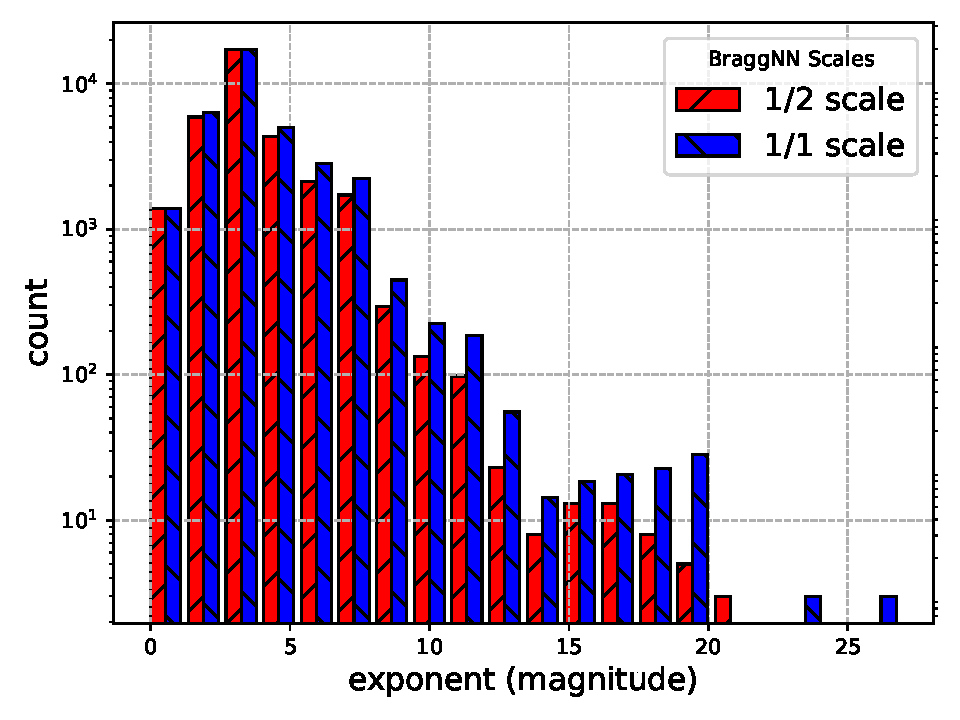
\includegraphics[width=\columnwidth]{figures/exp_hist}
	\caption{Range of exponent values for BraggNN weights.}\label{fig:numexp}
\end{figure}
With this in mind, we deploy BraggNN using quarter precision floats, i.e., using 4 bits to represent the exponent and 4 bits to represent the mantissa.
There is ample prior that shows 8-bit floating point is adequate during training and inference~\cite{https://doi.org/10.48550/arxiv.1812.08011, https://doi.org/10.48550/arxiv.2206.02915, https://doi.org/10.48550/arxiv.2001.05674}.
This produces floating point arithmetic cores that use fewer registers, LUTs, and having smaller wire delays, again leading to a reduction in overall complexity and end to end latency.
